\documentclass[aspectratio=1610]{beamer}

\usepackage[ngerman]{babel}
\usepackage[utf8]{inputenc}
\usepackage[absolute,overlay]{textpos}
\usepackage{xcolor}

\definecolor{black}{HTML}{3C3C3C}
\definecolor{green}{HTML}{BBE08C}

\mode<presentation>
{
  \usetheme[compress]{Torino}
}

\newcommand{\concept}[2]{
  \begin{block}{#1}
    \pause
    #2
  \end{block}
}

\newcommand{\pattern}[2]{
  \begin{alertblock}{Problem}
    #1
  \end{alertblock}
  \pause
  \begin{exampleblock}{Lösung}
    #2
  \end{exampleblock}
}

\newcommand{\boxx}[1]{
  \colorbox{black}{
    \color{green}{#1}
  }
}

\newcommand{\photoby}[3]{
  \begin{textblock*}{\paperwidth}[0.25,0](\textwidth,\textheight)
    \raggedright{
      \boxx{
        \tiny{
          Foto von \href{#2}{#1} (#3)
        }
      }
    }
  \end{textblock*}
}

\AtBeginSubsection[]{
  \begin{frame}
    \tableofcontents[currentsection, currentsubsection]
  \end{frame}
}


\title{Festplatten-Crypto mit LUKS}

\author[Mic]{Mic \flq nomaster@chaosdorf.de\frq}

\institute[chaosdorf]{Chaos Computer Club Düsseldorf / Chaosdorf e.V.}

\date[]{Chaosdorf, 17.11.2012}

\begin{document}

  \begin{frame}
    \titlepage
  \end{frame}

  \begin{frame}{Wozu?}
    \begin{itemize}
      \item{Erhöhter Zugriffsschutz}
      \pause
      \item{Schutz vor Datendiebstahl}
      \pause
      \item{Vereinfacht Weiterverwendung von Datenträgern}
    \end{itemize}
  \end{frame}

  \begin{frame}{Warum?}
    \begin{itemize}
      \item{Kompatibilität durch Standardisierung}
      \pause
      \item{Sicher gegen bekannte Angriffe}
      \pause
      \item{Mehrere Schlüssel unterstützt}
      \pause
      \item{Passphrase kann zurückgezogen werden}
    \end{itemize}
  \end{frame}

  \begin{frame}{Wie?}
    \begin{itemize}
      \item{cryptsetup auf der Kommadozeile}
      \pause
      \item{Integriert in Desktop-Umgebungen}
      \pause
      \item{Windows- und OSX-Implementierungen verfügbar}
    \end{itemize}
  \end{frame}

  \begin{frame}
    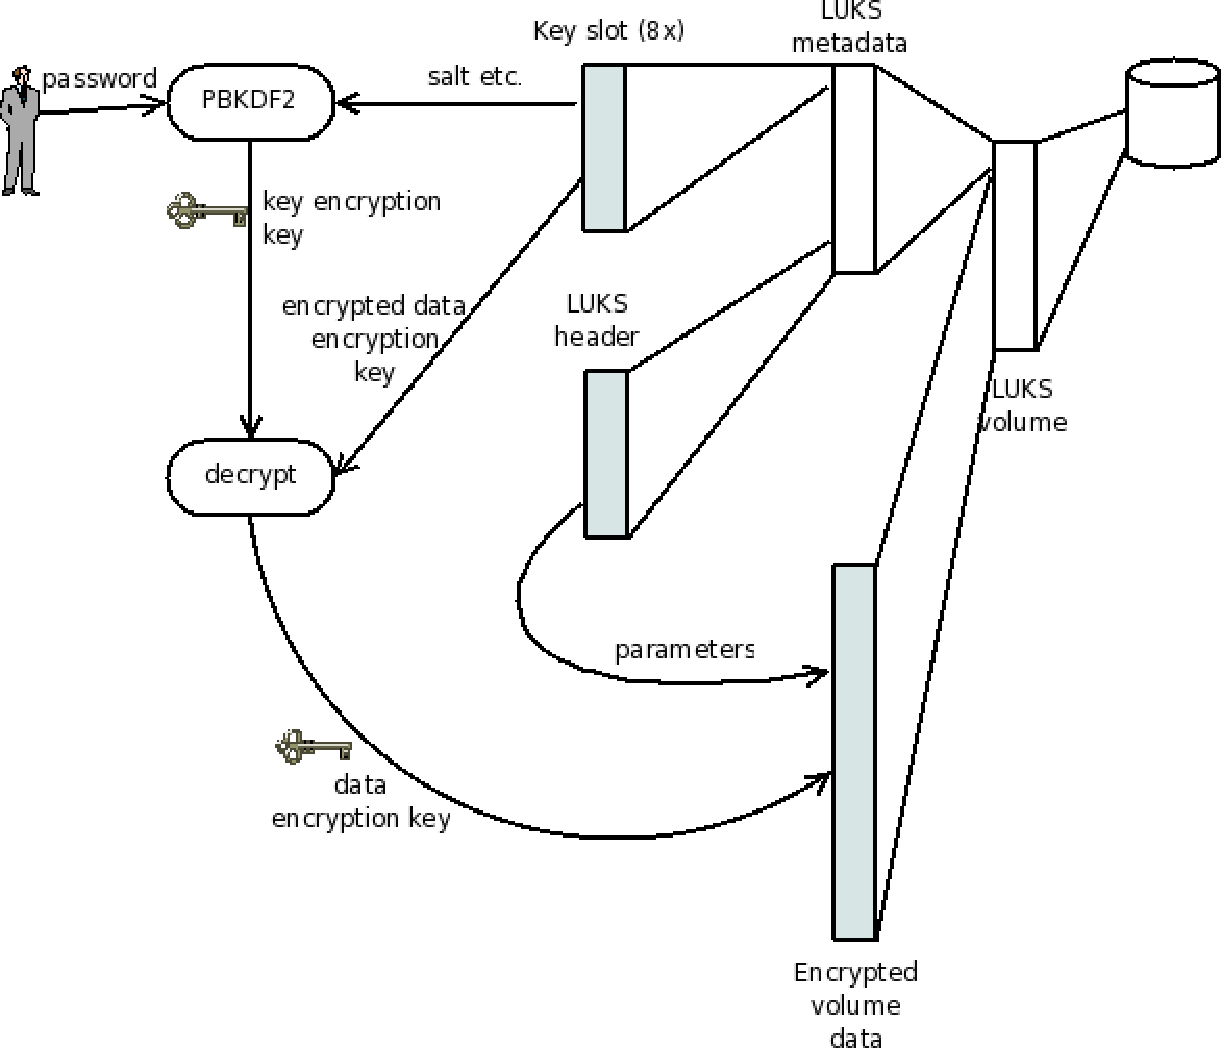
\includegraphics[height=\textheight]{overview.pdf}
  \end{frame}

  \begin{frame}{WTF?}
    \begin{itemize}
      \item{Einfach: Bei der Ubuntu-Installation auswählbar}
      \pause
      \item{Stabil: Geht auch ohne Klickibunti-Gedöns}
      \pause
      \item{Schnell: Verlangsamung minimal, weil integriert in Linux}
      \pause
      \item{Vertrauenswürdig: Freie Software, Quelltext einsehbar}
    \end{itemize}
  \end{frame}

  \begin{frame}{moar?}
    \begin{itemize}
      \item{Ubuntu Linux ''Alternate'' Installationsmedium}
      \pause
      \item{LUKS FAQ für mehr Informationen (englisch)}
      \pause
      \item{Mit USB-Stick testen (heute Workshop!)}
    \end{itemize}
  \end{frame}

  \begin{frame}{genug!}
    \begin{itemize}
      \item{follow, flattr, socialize @nomaster}
      \item{mail nomaster@chaosdorf.de}
    \end{itemize}
  \end{frame}

\end{document}
